\scalebox{0.9}{
    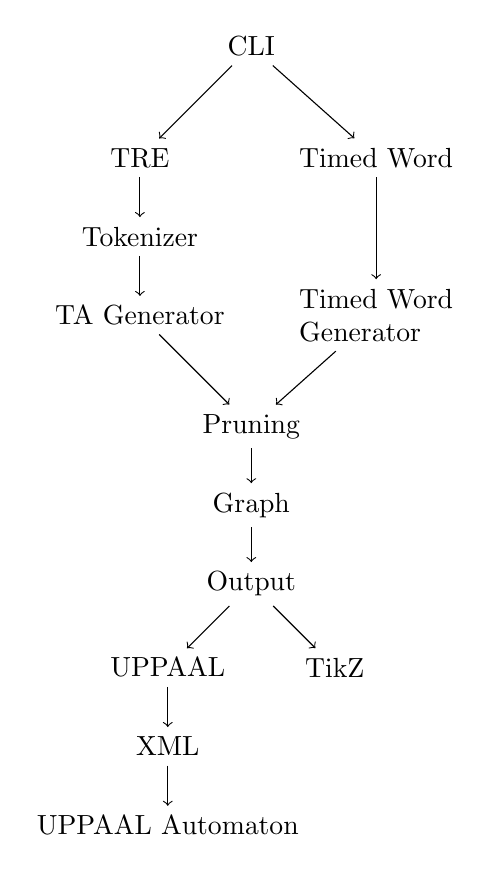
\begin{tikzpicture}[node distance = 1cm, auto]
        \node (CLI) {CLI};
        
        \node (TRE) [node distance = 2cm, below left of = CLI] {TRE};
        \node (TimedWord) [node distance = 3cm, right of = TRE] {Timed Word};
        \node (Tokenizer) [below of = TRE] {Tokenizer};
        \node (TAGenerator) [below of = Tokenizer] {TA Generator};
        \node (Pruning) [node distance = 2cm, below right of = TAGenerator] {Pruning};
        \node (Graph) [below of = Pruning] {Graph};
        \node (Output) [below of = Graph] {Output};
        \node (UPPAAL) [node distance = 1.5cm, below left of = Output] {UPPAAL};
        \node (XML) [below of = UPPAAL] {XML};
        \node (UPPAALAutomaton) [below of = XML] {UPPAAL Automaton};
        \node (TikZ) [node distance = 1.5cm, below right of = Output] {TikZ};
        \node (TimedWordGenerator) [node distance = 3cm, right of = TAGenerator,  align=left] {Timed Word\\Generator};
    
        \draw[->] (CLI) -- (TRE);
        \draw[->] (TRE) -- (Tokenizer);
        \draw[->] (Tokenizer) -- (TAGenerator);
        \draw[->] (TAGenerator) -- (Pruning);
        \draw[->] (Pruning) -- (Graph);
        \draw[->] (Graph) -- (Output);
        \draw[->] (Output) -- (UPPAAL);
        \draw[->] (UPPAAL) -- (XML);
        \draw[->] (XML) -- (UPPAALAutomaton);
        \draw[->] (Output) -- (TikZ);
        \draw[->] (CLI) -- (TimedWord);
        \draw[->] (TimedWord) -- (TimedWordGenerator);
        \draw[->] (TimedWordGenerator) -- (Pruning);
    \end{tikzpicture}
}
\label[figure]{fig:TREATdiagram}
